\section{Examples}

\subsection{How to run examples}

To run some examples you have to navigate into the \emph{prescient\_gosm} repository. There you  will find a folder called \emph{examples}. Navigate into this folder as well. If you want to run examples with the CAISO data, run the command:\\

\begin{figure}[H]
	\begin{framed}
		runner.py multiple\_sources\_gosm\_test/CAISO/CAISO\_populator\_mc.txt
	\end{framed}
\end{figure}

After that you will find the output in the directory \emph{multiple\_sources\_gosm\_test/CAISO/caiso\_output}.\\

It is a little bit trickier to run some examples with BPA data. First of all, you will  have to change some code. Inside the \emph{prescient\_gosm} repo, navigate to \emph{prescient\_gosm/markov\_chains}. Then edit the script \emph{markov\_populator.py} in the following way: In the function \emph{multiple\_sources} search for the part introduced by the comments "Adding some noise for testing purposes. (If theres real data available for one source)". Right after this comment there is a for-loop, which is commented out with three quotation marks. Delete these before and after the for-loop.\\

\begin{figure}[H]
	\centering
	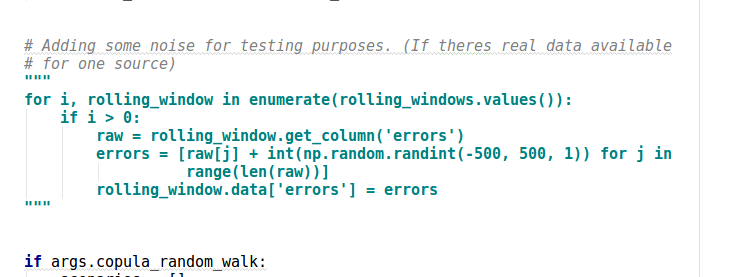
\includegraphics[width=0.9\textwidth]{code.png}
	\caption{The part of the code where you have to delete the quotation marks.}
\end{figure}

You have to do this, because there is only one real data set available for BPA, so we have to add some noise to this set to generate a  different data set which can be used as the second, third, etc, source. After this is done, you have to navigate again in the directory \emph{prescient\_gosm/examples} and run the following command:\\

\begin{figure}[H]
	\begin{framed}
		runner.py multiple\_sources\_gosm\_test/BPA/BPA\_populator\_mc.txt
	\end{framed}
\end{figure}

After that you will find the output in the directory \emph{multiple\_sources\_gosm\_test/BPA/bpa\_output}.
\textbf{Do not forget to add the quotation marks inside the code before you are running the script with CAISO data!}

\clearpage

\subsection{Example files}

\textbf{CAISO}

\begin{figure}[H]
	\begin{framed}
		command/exec populator.py\\
		
		-{}-start-date 2014-10-03-15:00
		
		-{}-end-date 2014-10-03-15:00\\
		
		-{}-load-scaling-factor 0.045\\
		
		-{}-output-directory multiple\_sources\_gosm\_test/CAISO/caiso\_output
		
		-{}-scenario-creator-options-file multiple\_sources\_gosm\_test/CAISO/CAISO\_scenario\_creator\_mc.txt
		
		-{}-sources-file multiple\_sources\_gosm\_test/CAISO/caiso\_sourcelist.txt
		
		-{}-allow-multiprocessing 0
		
		-{}-traceback
	\end{framed}
	\caption{CAISO\_populator\_mc.txt}
\end{figure}

\begin{figure}[H]
	\begin{framed}
		command/exec scenario\_creator.py\\
		
		-{}-use-markov-chains
		
		-{}-copula-random-walk
		
		-{}-planning-period-length 10H
		
		
		\# Options regarding file in- and output:
		
		-{}-sources-file multiple\_sources\_gosm\_test/CAISO/caiso\_sourcelist.txt
		
		-{}-output-directory multiple\_sources\_gosm\_test/CAISO/output\_scenario\_creator
		
		-{}-scenario-template-file multiple\_sources\_gosm\_test/CAISO/caiso\_simple\_nostorage\_skeleton.dat
		
		-{}-tree-template-file multiple\_sources\_gosm\_test/TreeTemplate.dat
		
		-{}-reference-model-file ../models/knueven/ReferenceModel.py
		
		-{}-number-scenarios 1\\
		
		\# General options:
		
		-{}-scenario-day 2015-06-30\\
		
		-{}-wind-frac-nondispatch=0.50
	\end{framed}
	\caption{CAISO\_scenario\_creator\_mc.txt}
\end{figure}

\begin{figure}[H]
	\centering
	\begin{framed}
		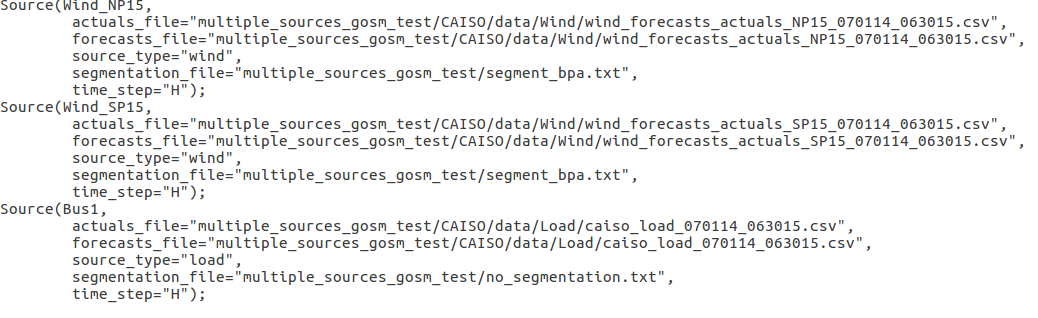
\includegraphics[width=0.9\textwidth]{caiso_sourcelist.png}
	\end{framed}
	\caption{caiso\_sourcelist.txt}
\end{figure}

\textbf{BPA}\\

\begin{figure}[H]
	\begin{framed}
		command/exec populator.py\\
		
		-{}-start-date 2013-02-03-03:00
		
		-{}-end-date 2013-02-03-03:00\\
		
		-{}-load-scaling-factor 0.045\\
		
		-{}-output-directory multiple\_sources\_gosm\_test/BPA/bpa\_output
		
		-{}-scenario-creator-options-file multiple\_sources\_gosm\_test/BPA/BPA\_scenario\_creator\_mc.txt
		
		-{}-sources-file multiple\_sources\_gosm\_test/BPA/bpa\_sourcelist\_bus1.txt\\
		
		-{}-allow-multiprocessing 0\\
		
		-{}-traceback
	\end{framed}
	\caption{BPA\_populator\_mc.txt}
\end{figure}

\begin{figure}[H]
	\begin{framed}
		command/exec scenario\_creator.py\\
		
		-{}-use-markov-chains
		
		-{}-copula-random-walk
		
		-{}-planning-period-length 10H\\
		
		\# Options regarding file in- and output:
		
		-{}-sources-file multiple\_sources\_gosm\_test/BPA/bpa\_sourcelist\_bus1.txt
		
		-{}-output-directory multiple\_sources\_gosm\_test/BPA/output\_scenario\_creator
		
		-{}-scenario-template-file multiple\_sources\_gosm\_test/BPA/simple\_nostorage\_skeleton.dat
		
		-{}-tree-template-file multiple\_sources\_gosm\_test/TreeTemplate.dat
	
		-{}-reference-model-file ../models/knueven/ReferenceModel.py
		
		-{}-number-scenarios 1\\
		
		\# General options:
		
		-{}-scenario-day 2015-06-30\\
		
		-{}-wind-frac-nondispatch=0.50
	\end{framed}
	\caption{BPA\_scenario\_creator\_mc.txt}
\end{figure}

\begin{figure}[H]
	\centering
	\begin{framed}
		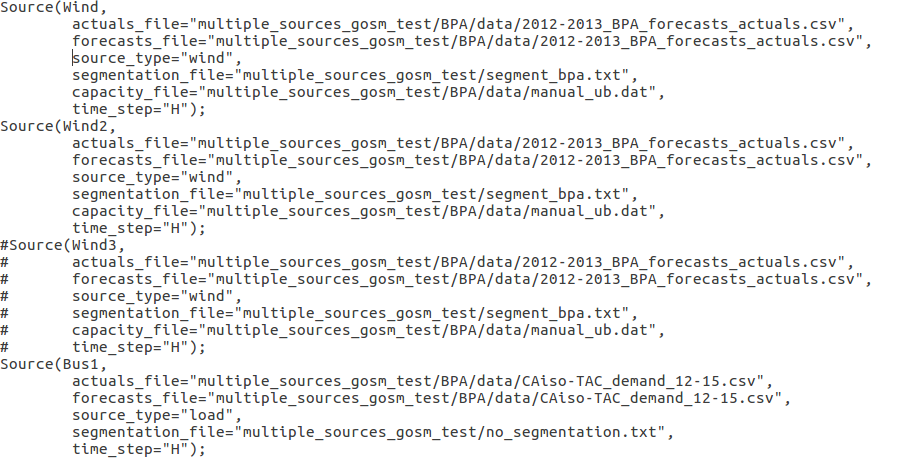
\includegraphics[width=0.9\textwidth]{bpa_sourcelist_bus1.png}
	\end{framed}
	\caption{bpa\_sourcelist\_bus1.txt}
\end{figure}




